\documentclass{article}
\usepackage{graphicx} % Required for inserting images
\usepackage{amsfonts}
\usepackage{float}

\title{24.06.25 Bug Discussion}
\author{Xun Zhang \quad \quad Bingsheng Zhang \\ 
Zhejiang University, CHN \\
22221024@zju.edu.cn \quad bingsheng@zju.edu.cn}

\date{June 25 2024}
\begin{document}

\maketitle

\section{BLS12-381 and Jubjub}

\subsection{BLS12-381}


The parameter of curve is:$\mathbf{z = -0xd201000000010000}$ (hexadecimal): low hamming weight, few bits set to $1$.

Field modulus: $q = \frac{1}{3}(z-1)^2(z^4 - z^2 + 1) + z$, $381$-bit:

$\mathbf{q = 0x1a0111ea397fe69a4b1ba7b6434bacd764774b84f38512bf6730d2a0f6b0f62} \\
\mathbf{41eabfffeb153ffffb9feffffffffaaab}$





Subgroup size: $r = (z^4 - z^2 + 1)$, $255$-bit:

  $\mathbf{r = 0x73eda753299d7d483339d80809a1d80553bda402fffe5bfeffffffff00000001}$


And the form of curve BLS12-381 is:
\[
E(\mathbb{F}_q) := y^2 = x^3 + 4
\]


\subsection{Jubjub}
Jubjub is an elliptic curve of the twisted Edward's form. It is defined over finite field $\mathbb{F}_q$ where

$\mathbf{q = 0x73eda753299d7d483339d80809a1d80553bda402fffe5bfeffffffff00000001}$

with a subgroup of order $r$ and cofactor $8$.

$\mathbf{r = 0x0e7db4ea6533afa906673b0101343b00a6682093ccc81082d0970e5ed6f72cb7}$

Let $d = -(10240/10241)$, the Jubjub curve is defined as follows:

$$E_{d}: -u^2 + v^2 = 1 + du^2v^2.$$

$\mathbb{F}_q$ is chosen to be the scalar field of BLS12-381 curve construction.


\subsection{Relations in Code}

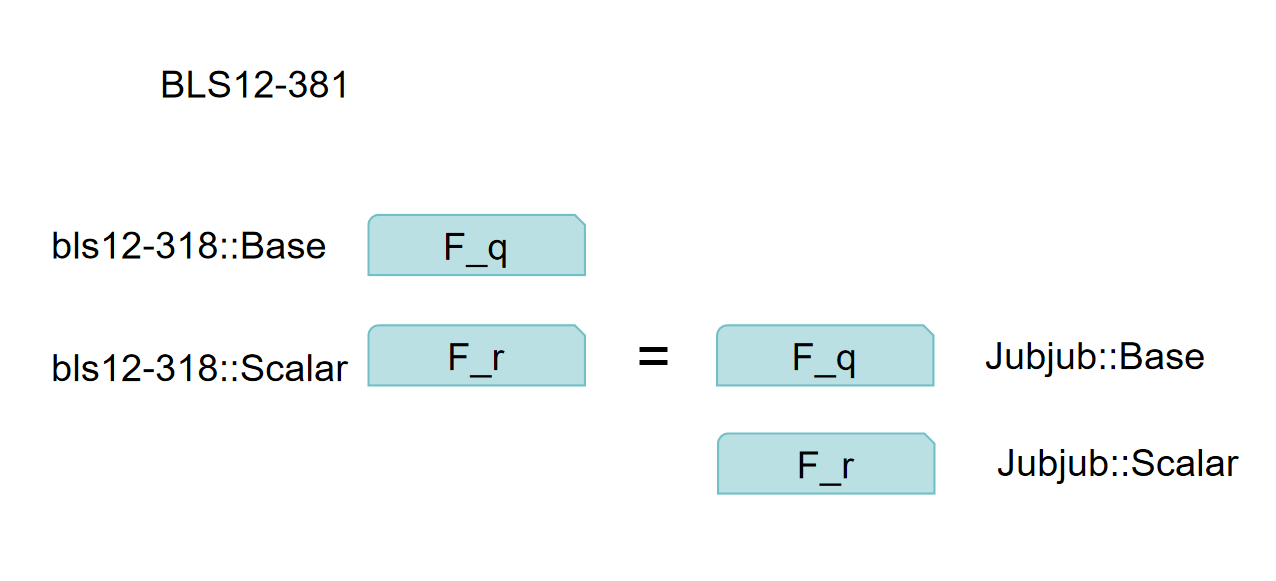
\includegraphics[width=1\linewidth]{base_scalar.png}


\section{Bug Analysis}

\subsection{Description}

We test the simplest schnorr multi-signature scheme:

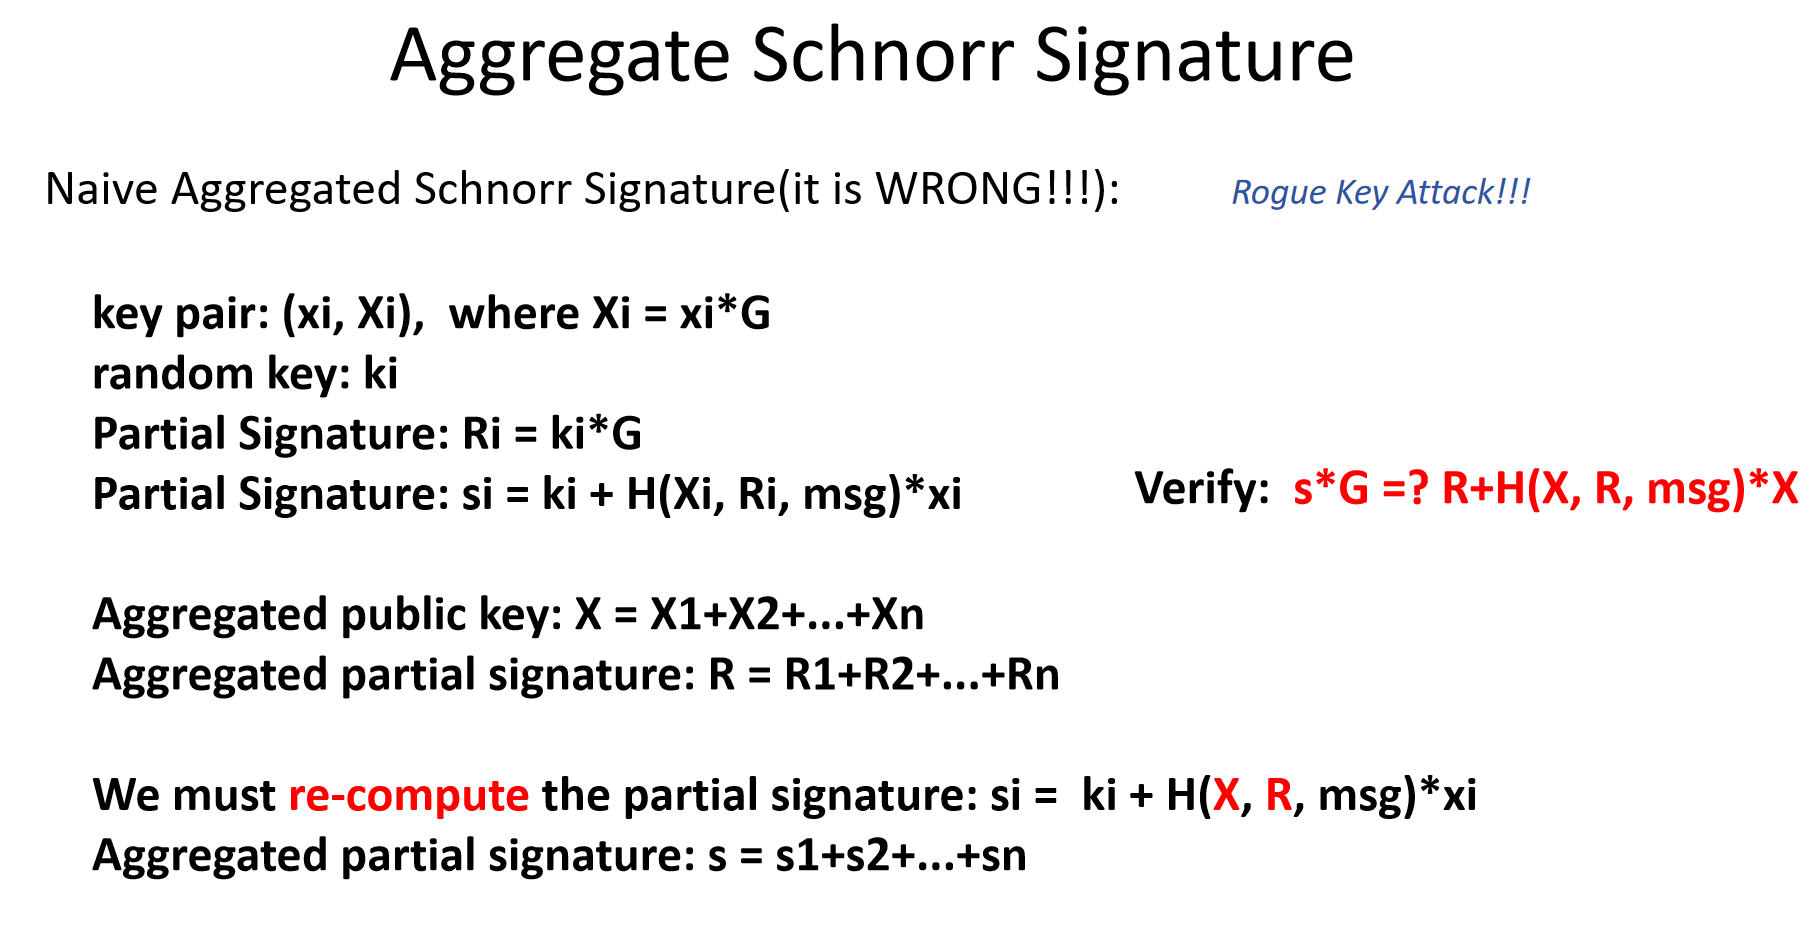
\includegraphics[width=1\linewidth]{schnorr multisig v1.png}

And find that when the random seed changes, the test results also change.
We use random Chacha20 as a rng.
\begin{itemize}
    \item num of parties: 16, random seed = [0u8;32]. Test \textbf{pass}.
    \item num of parties: 17, random seed = [0u8;32]. Test \textbf{fail}.
    \item num of parties: 17, random seed = [111u8;32]. Test \textbf{pass}.
    \item num of parties: 16, random seed = [111u8;32]. Test \textbf{fail}.
\end{itemize}

The failure happens in below equation(it is implemented in other form in code):

\[
s*G = R + H(R,X,msg)*X
\]

If we add the constraint for public inputs, the situation becomes more complex. We add three constraints:
\begin{enumerate}
    \item aggregated pk
    \item aggregated signature \textbf{R} in (R,s)
    \item aggregated signature \textbf{s} in (R,s)
\end{enumerate}

Note that the aggregated signature scalar \textbf{s} will be transformed in base field of Jubjub(which is scalar filed of BLS12-381).

And the two coordinates of aggregated signature \textbf{R} is also in base field of Jubjub.

And the test results of these three public inputs are:

\begin{enumerate}
    \item aggregated pk: always \textbf{pass} the test.
    \item aggregated signature \textbf{R}: always \textbf{pass} the test.
    \item aggregated signature \textbf{s}: Always \textbf{fails}.
\end{enumerate}

It is very strange that since the aggregated signature \textbf{s} always fails the test, how can the test pass(without public input constraint).


See screen shot of code:

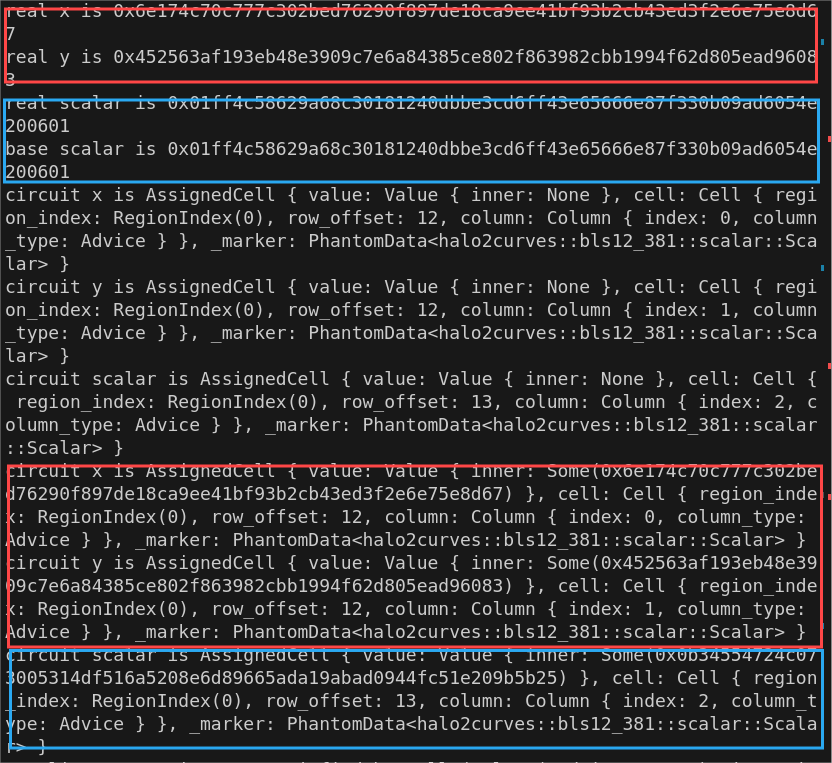
\includegraphics[width=1\linewidth]{bug screen shot.png}

\subsection{A Possible Reason}

I think the a possible reason is that there is no struct for a \textbf{Scalar} value in Jubjub curve.

Since the \textbf{Scalar} is much smaller than \textbf{Base}, it is handy to use a \textbf{Base} type value as \textbf{Scalar}. See picture below:

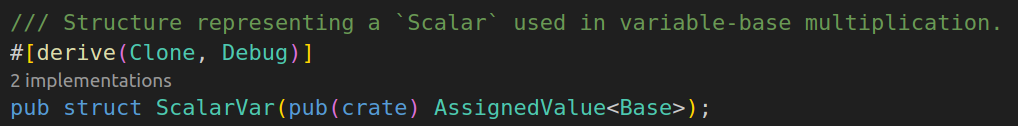
\includegraphics[width=1\linewidth]{scalarvar.png}

In this way, there will be bugs in the calculation of signature \textbf{s}:

\[
s = s_1 + s_2 + \ldots + s_n
\]

This is because the addition of partial signature \textbf{$s_i$} will be under the modulus of \textbf{Jubjub::Base}, but what we need is the modulus of \textbf{Jubjub::Scalar}.

\subsection{Solution}

We just do a modular arithmetic on every addition. Here we multiplexing the code of checking equality:
\[
s*G = R+H(X, R, msg)*X
\]

The challenge, or $H(X, R, msg)$ will be reduces to \textbf{Scalar} filed to multiply \textbf{X}. We do the same thing to the addition results of every two $s_i$. See code below:

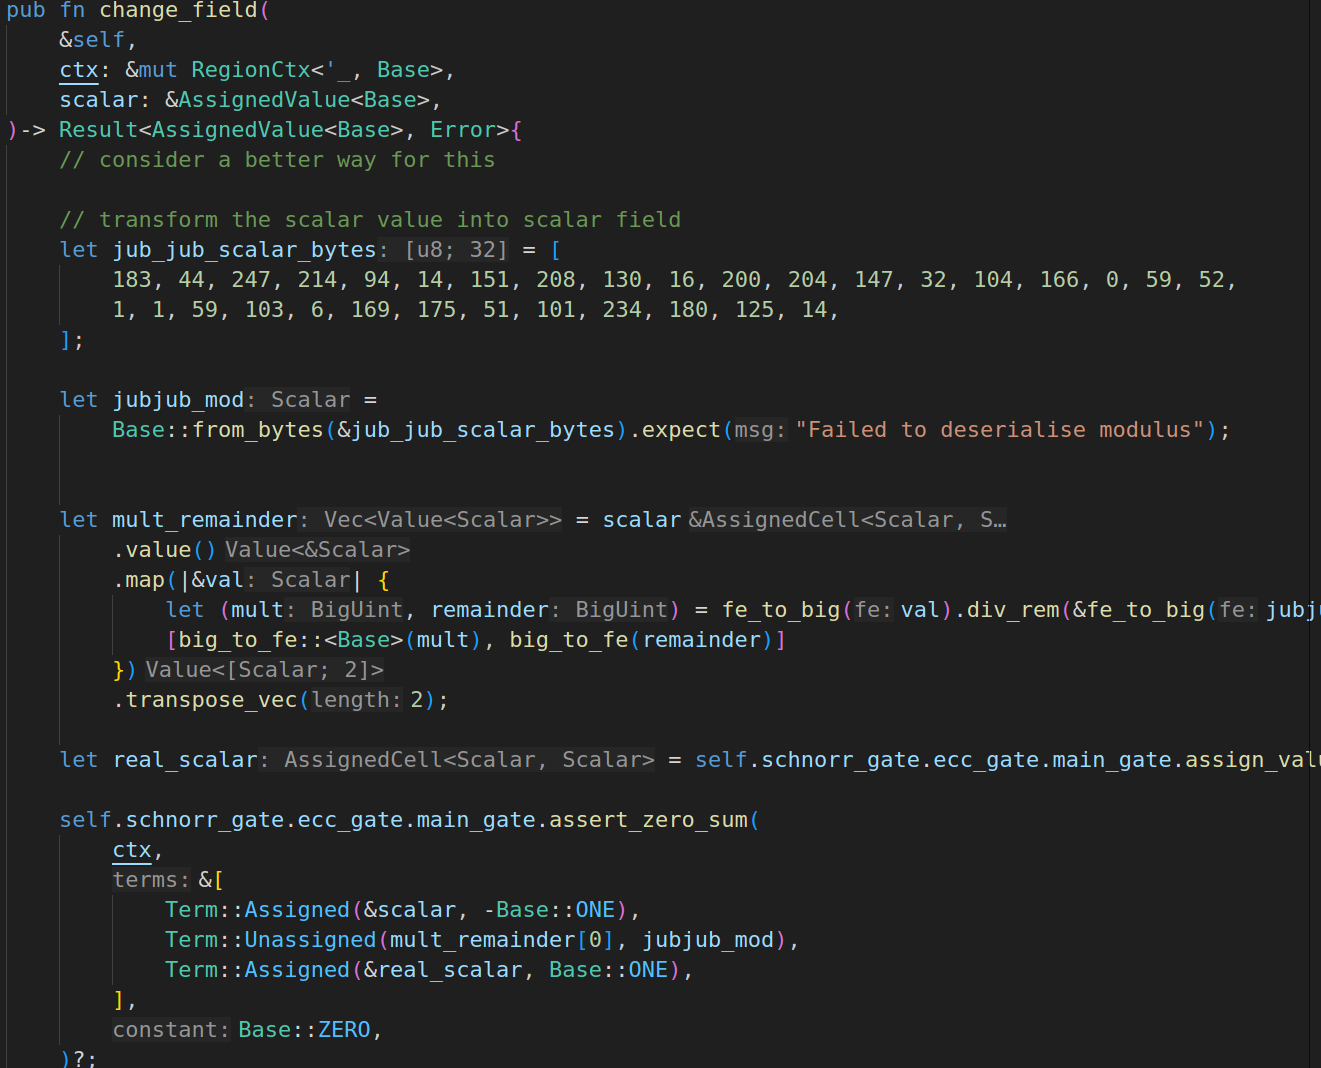
\includegraphics[width=1\linewidth]{change_field.png}

And this will cost a constraint:
\[
scalar(base filed) = mult\_remainder * jubjub\_mod + real_scalar(scalar field)
\]

\section{Benchmark}

The Bug above will influence the performance of SNARK-based Aggregated Schnorr Signature scheme. Note that it is the \textbf{original} implementation of Aggregated Schnorr signature, without any optimization.

\begin{table}[H]
    \centering
    \begin{tabular}{c|c} \hline
        Setting & Proving Time \\ \hline
         k = 13, n = 5& 0.8408s  \\ \hline
         k = 14, n = 8& 1.3719s \\ \hline
         k = 15, n = 14& 2.4313s \\ \hline
         k = 16, n = 20& 4.4653s \\ \hline
         k = 17, n = 32& 8.3078s \\ \hline
         k = 19, n = 72& 30.616s \\ \hline
    \end{tabular}
    \caption{Proving time of Aggregated Schnorr Signature}
    \label{tab:my_label}
\end{table}


This proof of concept implementation mainly proves the following core components of signature scheme:
\begin{enumerate}
    \item $R = R_1 + R_2 + ... + R_n$
    \item $a_i = H(L || X_i)$ for all $X_i$, where $L = (X_1, X_2, ... , X_n)$
    \item $X = a_1*X_1 + a_2*X_2 +...+ a_n*X_n$
    \item $s = s_1 + s_2 + ... + s_n$
    \item $s*G =? R+H(X, R, msg)*X$
\end{enumerate}


\section{Merkle Tree Root Proof}

We use the Rescue hash function to build a 2-arity merkle tree, to prove that the correctness of the root. Here is the benchmark.

n is the number of leaves.

\begin{table}[H]
    \centering
    \begin{tabular}{c|c} \hline
        Setting & Proving Time \\ \hline
         k = 13, n = 16& 0.6570s  \\ \hline
         k = 14, n = 64& 1.1433s \\ \hline
         k = 16, n = 256& 3.8133s \\ \hline
         k = 18, n = 1024& 13.763s \\ \hline
         k = 19, n = 2048& 26.243s \\ \hline
    \end{tabular}
    \caption{Proving time of Merkle Tree Root}
    \label{tab:my_label}
\end{table}


\section{An Optimized Aggregated Schnorr Signature}

Consider the real workflow of a aggregated signature scheme, it is reasonable to add the membership-proof feature into the workflow.

The optimized Aggregated Schnorr signature scheme has two set of public keys. One of which is the public keys used to "sign" the message, the other one is the public keys participate in the merkle tree root proving(as a member of leaves).
\begin{enumerate}
    \item  $R = R_1 + R_2 + ... + R_n$
    \item $(X_1, X_2, ... , X_n) \in PK$, where $PK = (X_1, X_2, ... , X_n, NX_1, NX_2, ... , NX_m)$
    \item $a_i = H(L || X_i)$ for all $X_i$, where $L = ROOT(X_1, X_2, ... , X_n, NX_1, NX_2, ... , NX_m)$
    \item $X = a_1*X_1 + a_2*X_2 +...+ a_n*X_n$
    \item $s = s_1 + s_2 + ... + s_n$
    \item $s*G =? R+H(X, R, msg)*X$
\end{enumerate}

Thus we need a efficient membership-proof technique to prove the \textbf{step 2}. We plan to use the Merkle tree path to prove the relation firstly.


\end{document}
